\documentclass[glossy]{beamer}
\useoutertheme{wuerzburg}
\useinnertheme[realshadow,corners=2pt,padding=2pt]{chamfered}
\usecolortheme{shark}

\usepackage{listings}

\usepackage{fancyvrb}
%\usepackage[scaled]{beramono} %sets the beramono font. Just comment this line to get the default font back

\usepackage{tikz}
\newcommand<>{\hover}[1]{\uncover#2{%
 \begin{tikzpicture}[remember picture,overlay]%
 \draw[fill,opacity=0.4] (current page.south west)
 rectangle (current page.north east);
 \node at (current page.center) {#1};
 \end{tikzpicture}}
}

\title{Arquitecturas y Organización de Computadoras I \\\line(1,0){320}}
% \author{\texorpdfstring{Author\newline\url{email@email.com}}{Author}}
%\author{Rafael Ignacio Zurita}
\institute{Rafael Ignacio Zurita \\ Departamento de Ingenieria de Computadoras - FAI - UNCOMA 2018 \\ Clase presencial 4}
%\date{\today}



\begin{document}




\begin{frame}
\maketitle
\end{frame}

\institute{Departamento de Ingenieria de Computadoras - FAI - UNCOMA \\ 2018}

\begin{frame}
\frametitle{Programa Analítico}
\textbf{UNIDAD I: Arquitectura y Organización de Computadoras}
 \\~\\
\textit{Formatos de instrucciones. Modos de direccionamiento. Tipos de instrucciones. Lenguaje ensamblador: directivas, operaciones, pseudo-operaciones, macros.} 
 \\~\\
\end{frame}


\begin{frame}
\frametitle{Temario}
\begin{itemize}
\item Operaciones (instrucciones) y el conjunto de instrucciones MIPS
\item Modos de direccionamiento
\item Lenguaje Máquina
\item Ensamblador
\item Traducción de declaraciones en C a lenguaje ensamblador
\end{itemize}
\end{frame}



\begin{frame}
\frametitle{Tipos de Instrucciones}
\begin{center}\textbf{Tipos Principales de Instrucciones}\end{center}
\begin{itemize}
\item Aritméticas y Lógicas
\begin{itemize}
\item Enteros
\item Punto Flotante
\end{itemize}
\item Instrucciones de transferencia de datos (memoria)
\begin{itemize}
\item Carga y Almacenamiento
\end{itemize}
\item Flujo de control
\begin{itemize}
\item Salto
\item Bifurcación condicional
\item Llamado y Retorno
\end{itemize}
\end{itemize}
\end{frame}



\begin{frame}[fragile]
\frametitle{Tipos de Instrucciones}
\begin{center}\textbf{Instrucciones aritméticas en MIPS}\end{center}
\begin{itemize}
\item Las instrucciones aritméticas y lógicas más comunes tienen 3 operandos
\item El orden de los operandos es fijo (el destino primero)
\item Ejemplo:
\end{itemize}

% \footnotesize
\begin{verbatim}

  Código C:        a = b + c;

  Código MIPS:     add $s0, $s1, $s2

(el compilador asocia a $s0, $s1 y $s2 a las variables a, b y c)

\end{verbatim}

\end{frame}



\begin{frame}[fragile]
\frametitle{Tipos de Instrucciones}
\begin{center}\textbf{Instrucciones aritméticas en MIPS}\end{center}

\begin{verbatim}

  Código C:        a = b + c + d;
                   e = f - a;

  Código MIPS:     add $t0, $s1, $s2
                   add $s0, $t0, $s3
                   sub $s4, $s5, $s0
\end{verbatim}
\begin{itemize}
\item Los operandos deben estar en registros, y existen sólo 32
\item Principio de diseño: Más pequeño es más rápido. Porqué? (viaje de las señales)
\end{itemize}
\end{frame}





\begin{frame}
\frametitle{Tipos de instrucciones en MIPS}
\begin{center}\textbf{Registros vs. Memoria}\end{center}

\begin{itemize}
\item Los operandos deben estar en registros, y existen sólo 32
\item El compilador asocia variables a registros
\item ¿Qué sucede con un programa con un montón de variables?
\end{itemize}
\begin{center}
\begin{figure}
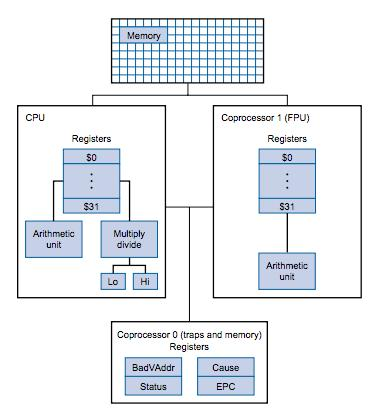
\includegraphics[scale=0.4]{organizacion-mips.jpg} 
\end{figure}
\end{center}
\end{frame}


\begin{frame}
\frametitle{Representación de datos a nivel máquina}
\textbf{Organización de la Memoria principal en MIPS}
\begin{itemize}
	\item $2^{32}$ bytes, con direcciones 0, 1, 2 ... 
	\item $2^{30}$ 4-bytes palabras, con direcciones 0, 4, 8 ... 
	\item Las direcciones de las palabras deben ser múltiplos de 4
\end{itemize}
	\begin{center}
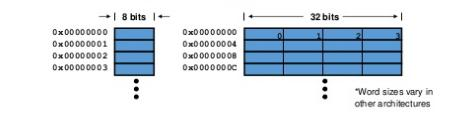
\includegraphics[scale=0.5]{memoria-mips.jpg} 
	\end{center}
\end{frame}


\begin{frame}[fragile]
\frametitle{Tipos de Instrucciones}
\begin{center}\textbf{Registros vs. Memoria}\end{center}

\begin{itemize}
\item Los operandos deben estar en registros, y existen sólo 32
\item El compilador asocia variables a registros
\item ¿Qué sucede con un programa con un montón de variables?
\end{itemize}
\end{frame}



\begin{frame}[fragile]
\frametitle{Tipos de Instrucciones}
\begin{center}\textbf{Asignación de Registros}\end{center}

\begin{itemize}
\item El compilador intenta asociar tantas variables a registros como sea posible
\item Algunas variables no pueden ser alocadas
\begin{itemize}
\item grandes arreglos (vectores)
\item variables accedidas con diferentes punteros
\item variables alocadas dinamicamente
\begin{itemize}
\item heap
\item stack
\end{itemize}
\end{itemize}
\item El compilador podría quedarse sin registros : \textbf{spilling}
\end{itemize}
\end{frame}



\begin{frame}[fragile]
\frametitle{Tipos de Instrucciones}
\begin{center}\textbf{Instrucciones de transferencia de datos}\end{center}

\begin{itemize}
\item Instrucciones de \textbf{Carga} y \textbf{Almacenamiento}
\item Ejemplo:
\end{itemize}
\begin{verbatim}

  Código C:        a[8] = h + a[8];

  Código MIPS:     lw  $t0, 32($s3)
                   add $t0, $s2, $t0
                   sw  $t0, 32($s3)
\end{verbatim}
\begin{itemize}
\item Las operaciones de carga y almacenamiento no tienen operandos destino (registro)
\item Recuerde: las operaciones aritméticas y lógicas operan sobre registros, no sobre elementos en la memoria!
\end{itemize}
\end{frame}




\begin{frame}
\frametitle{Formato de instrucciones en MIPS}
\begin{center}\textbf{Un ejemplo completo de traducción de C al lenguaje de la máquina}\end{center}
\begin{itemize}
\item ¿Puede interpretar la asignación de variables y el por qué del código en lenguaje ensamblador?
\end{itemize}
	\begin{center}
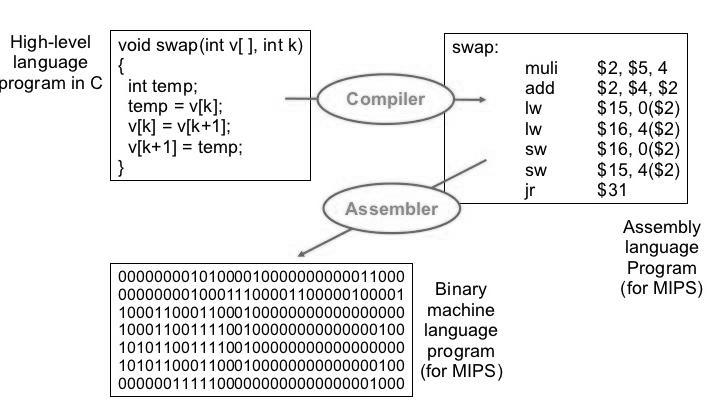
\includegraphics[scale=0.4]{below2.jpg} 
	\end{center}
\end{frame}




\begin{frame}[fragile]
\frametitle{Tipos de Instrucciones}
\begin{center}\textbf{Repaso}\end{center}

\begin{itemize}
\item MIPS
\begin{itemize}
\item Cargamos palabras (words) pero utilizamos direccionamiento del primer byte
\item Las instrucciones aritméticas y lógicas operan unicamente con registros
\end{itemize}
\end{itemize}
\begin{verbatim}

  Instrucción            Significado

  add $s1, $s2, $s3      $s1 = $s2 + $s3
  sub $s1, $s2, $s3      $s1 = $s2 - $s3
  lw $s1, 100($s2)       $s1 = MEMORIA[$s2+100]
  sw $s1, 100($s2)       MEMORIA[$s2+100] = $s1
\end{verbatim}
\end{frame}


\begin{frame}[fragile]
\frametitle{Lenguaje Máquina}
\begin{center}\textbf{Formato de Instrucciones en MIPS}\end{center}
\begin{itemize}
\item Las instruccciones, como los registros y la palabra, son de 32-bits
\begin{itemize}
\item Los registros están numerados en el código máquina: del 0 al 31
\end{itemize}
\end{itemize}
	\begin{center}
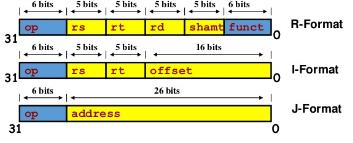
\includegraphics[scale=0.7]{formato.jpg} 
	\end{center}
\end{frame}



\begin{frame}[fragile]
\frametitle{Tipos de Instrucciones}
\begin{center}\textbf{Instrucciones de transferencia de Control}\end{center}

\begin{itemize}
\item Instrucciones para realizar decisiones
\begin{itemize}
\item Alterar el flujo de control de ejecución
\item y por lo tanto, cambiar la "próxima" instrucción a ser ejecutada
\end{itemize}
\item Instrucciones de bifurcación condicional en MIPS
\begin{verbatim}
                bne $t0, $t1, label
                beq $t0, $t1, label
\end{verbatim}
\item Ejemplo:
\begin{verbatim}
   Código en C:      if (i == j)  h = i + j;

   Código en MIPS:         bne $s0, $s1, label
                           add $s3, $s0, $s1
                     label: ...
\end{verbatim}
\end{itemize}
\end{frame}




\begin{frame}[fragile]
\frametitle{Tipos de Instrucciones}
\begin{center}\textbf{Instrucciones de transferencia de Control}\end{center}

\begin{itemize}
\item Instrucciones de salto incondicional
\begin{itemize}
\item j  label
\end{itemize}
\item Ejemplo:
\begin{verbatim}
   Código en C:      if (i != j)  
                           h = i + j;
                     else
                           h = i - j;


   Código en MIPS:         beq $s4, $s5, lab1
                           add $s3, $s4, $s5
                           j lab2
                     lab1: sub $s3, $s4, $s5
                     lab2:
\end{verbatim}
\end{itemize}
\end{frame}




\begin{frame}[fragile]
\frametitle{Tipos de Instrucciones}
\begin{center}\textbf{Repaso}\end{center}

\footnotesize
\begin{verbatim}

Instrucción            Significado

add $s1, $s2, $s3      $s1 = $s2 + $s3
sub $s1, $s2, $s3      $s1 = $s2 - $s3
lw $s1, 100($s2)       $s1 = MEMORIA[$s2+100]
sw $s1, 100($s2)       MEMORIA[$s2+100] = $s1
bne $s4, $s5, Etiq     Próx. instr. está en Etiq si $s4 es distinto a $s5
beq $s4, $s5, Etiq     Próx. instr. está en Etiq si $s4 es igual a $s5
j Etiqueta             Próx. instr. está en Etiqueta

\end{verbatim}
\end{frame}


\begin{frame}[fragile]
\frametitle{Tipos de Instrucciones}
\begin{center}\textbf{Instrucciones de transferencia de Control}\end{center}

\begin{itemize}
\item Salto condicional: bne, beq
\item ¿Qué sucede con saltar si es menor qué?
\item Nueva instrucción:
\begin{verbatim}
   slt $t0, $s1, $s2

Significado:      if $s1 < $s2 then
                      $t0 = 1
                  else
                      $t0 = 0
\end{verbatim}
\item Puede ser utilizada para construir \begin{verbatim}"blt $s1, $s2, Etiqueta"\end{verbatim}
\begin{itemize}
\item Se pueden construir estructuras de control de ejecución generales
\end{itemize}
\item El ensamblador necesita utilizar un registro \textit{temporal}
\begin{itemize}
\item Convención de uso de registros
\end{itemize}
\end{itemize}
\end{frame}


\begin{frame}
\frametitle{Modelo de programación MIPS}
        \begin{center}
        \textbf{Convención de uso de registros en MIPS}
 \\~\\

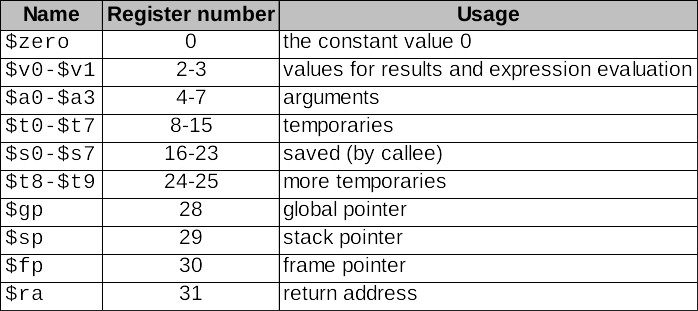
\includegraphics[scale=0.4]{convencion.jpg}

        \end{center}
\end{frame}


\begin{frame}[fragile]
\frametitle{Modelo de programación MIPS}
\begin{center}\textbf{Constantes}\end{center}

\begin{itemize}
\item Pequeñas constantes son utilizadas muy frecuentemente (50 por ciento de los operandos son constantes)
\begin{verbatim}
Ejemplo:   a = a + 5;
           b = b + 1 ;
           c = c * 2 + 1;
\end{verbatim}
\item ¿Soluciones? 
\begin{itemize}
\item Poner las constantes típicas (1, 2, 10) en memoria y cargarlas
\item Crear registros cableados en hardware con un valor (hard-wired). Como el registro zero
\item o .....
\end{itemize}
\item Colocar las constantes como parte de las Instrucciones (MIPS)
\begin{verbatim}
Ejemplo:   addi $29, $29 + 5
           addi $8, $8, 1
           andi $29, $29, 6
           ori $9, $9, 4
\end{verbatim}
\end{itemize}
\end{frame}




\begin{frame}[fragile]
\frametitle{Modelo de programación MIPS}
\begin{center}\textbf{¿Qué sucede con grandes Constantes?}\end{center}

\begin{itemize}
\item Las instrucciones son de 32-bits, por lo que no es posible colocar una constantes de 32-bits dentro de la instrucción.
\item Solución: para cargar una constante de 32-bit en un registro se utilizan dos instrucciones
\begin{verbatim}
Ejemplo:   lui $t0, 0xAAAA
           ori $t0, 0xAAAA
\end{verbatim}
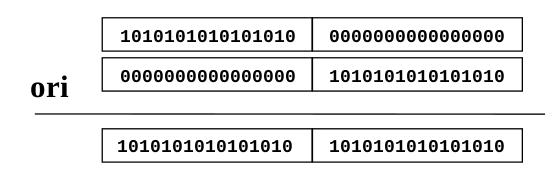
\includegraphics[scale=0.4]{ori.jpg}
\end{itemize}
\end{frame}


\begin{frame}[fragile]
\frametitle{Modelo de programación MIPS}
\begin{center}\textbf{Lenguaje Ensamblador vs. Lenguaje Máquina?}\end{center}

\begin{itemize}
\item El lenguaje ensamblador provee una representación simbólica conveniente
\begin{itemize}
\item Es mucho más sencillo que programar escribiendo números
\item Por ejemplo: el destino de una operación va primero
\end{itemize}
\item El lenguaje máquina es la verdadera realidad
\begin{itemize}
\item Por ejemplo: el destino ya no es lo primero que aparece en una operación va primero
\end{itemize}
\item El lenguaje ensamblador puede proveer \textbf{pseudoinstrucciones}
\begin{itemize}
\item Por ejemplo: \begin{verbatim}move $t0, $t1\end{verbatim}
\item sería implementadao utilizando:  \begin{verbatim}add $t0, $t1, $zero\end{verbatim}
\end{itemize}
\item Cuando se debe considerar la performance se deben contar las instrucciones reales
\end{itemize}
\end{frame}




\begin{frame}
\frametitle{Programación de la máquina: lenguaje ensamblador MIPS}
        \begin{center}
        \textbf{Conjunto básico de instrucciones MIPS}
        \end{center}
\begin{tabular}{cl}

\begin{tabular}{c}
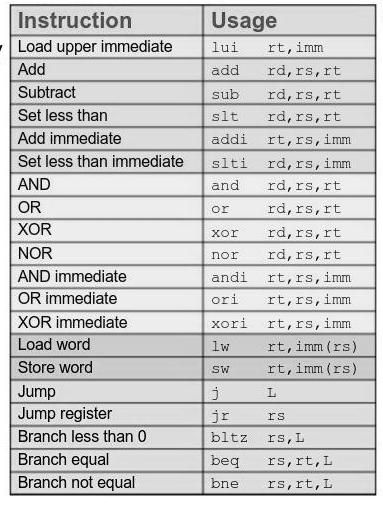
\includegraphics[height=5cm, width=4cm]{instrucciones-mips.jpg}

\end{tabular}
& \begin{tabular}{l}
\parbox{0.5\linewidth}{

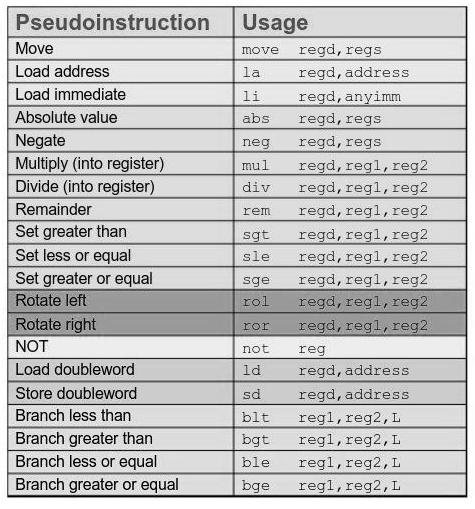
\includegraphics[height=5.2cm, width=4cm]{pseudoinstrucciones-mips2.jpg}
}
\end{tabular} \\

\end{tabular}
\end{frame}


\begin{frame}[fragile]
\frametitle{Modelo de programación MIPS}
\begin{center}\textbf{Resumen de la arquitectura MIPS}\end{center}
\begin{itemize}
\item Instrucciones sencillas de 32-bits de ancho
\item Muy estructurado, no hay necesidad de grandes variaciones
\item Confía en el compilador para ganar performance
\item Hay que ayudar al compilador cuando sea necesario
\item Únicamente 3 formatos de instrucciones
	\begin{center}
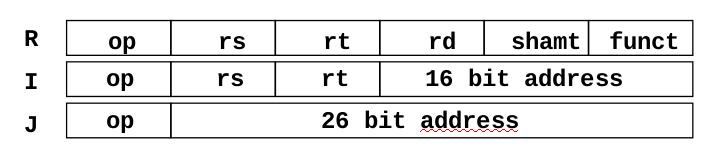
\includegraphics[scale=0.3]{formato2.jpg} 
	\end{center}
\item ¿Cómo programar mejor? (cantidad de variables, constantes)
\end{itemize}
\end{frame}


\begin{frame}[fragile]
\frametitle{Modos de direccionamiento}
\begin{itemize}
\item Los modos de direccionamiento son las diferentes formas de especificar un operando dentro de una instrucción (a nivel código máquina).
\item Es el CÓMO se especifican e interpretan las direcciones de memoria según las instrucciones
\item NO CONFUNDIR modos de direccionamiento con los formatos de direccionamiento permitidos al programar en lenguaje ensamblador
\item Absoluto, Inmediato, Directo por registro suelen ser los mas importantes
\end{itemize}
\end{frame}


\begin{frame}[fragile]
\frametitle{Modos de direccionamiento}
\begin{center}\textbf{Modos de direccionamiento en MIPS}\end{center}
	\begin{center}
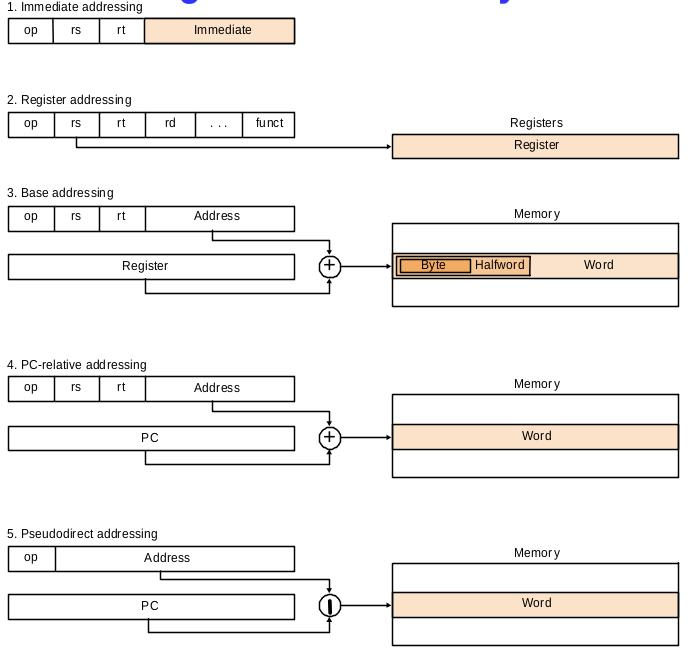
\includegraphics[scale=0.3]{modos-de-direccionamiento.jpg} 
	\end{center}
\end{frame}

\begin{frame}
 \frametitle{Consejos y preguntas}
\begin{center}
\begin{itemize}
\item  ¿Preguntas?
\end{itemize}
\end{center}
\end{frame}


\begin{frame}
 \frametitle{Bibliografía}
Libros
\begin{itemize}
\item Andrew S. Tanenbaum (2000), ORGANIZACIÓN DE COMPUTADORAS un enfoque estructurado, Editorial Prentice Hall. (10 copias en biblioteca)
\item David. Patterson John L. Hennessy (1995), ORGANIZACIÓN Y DISEÑO DE COMPUTADORES La interfaz hardware/software, McGraw-Hill (8 copias en biblioteca).
\end{itemize}
Contenido electrónico
\begin{itemize}
	\item \textbf{x86 assembly basis} Una introducción al lenguaje ensamblador x86. Disponible en PEDCO en formato PDF.
		\url{https://www.nayuki.io/page/a-fundamental-introduction-to-x86-assembly-programming}
\item Apuntes elaborados por la cátedra, disponibles en PEDCO para impresión (pdf) o lectura online (html)
\item Secciones de libros aptas para publicacion
\end{itemize}
\end{frame}


\end{document}
